\section{Transformer-based appraoches}
\label{sec:transformerBasedApproaches}

In recent years, other research fields have arisen.
Visual grounding tasks, for example, input text descriptions and try to localize the described objects in a scene \cite{openvocabularysurvey2024}.
Visual grounding can deal with semantic segmentation or bounding boxes.
One of the most promising approaches is Grounding DINO \cite{groundingdino2024}, which combines grounding and transformer-based detection in a single framework, achieving strong results in object detection benchmarks.
This framework cannot be used for segmentation tasks \cite{glipv22022}.
Grounding DINO achieves a speed of 8.37 FPS, which makes it too slow for real-time applications \cite{groundingdino2024}.
The model is trained on 64 NVIDIA A100 GPUs, far exceeding the resources available for this work.
Despite a strong performance in object detection benchmarks, there are several reasons why this model is not further considered.
This model is too slow for real-time applications; there is a lack of data to leverage this model's advantages fully, and it would not make sense to consider it for use on limited embedded devices.

\vspace{0.5cm}

Another concept is open vocabulary detection, which extends the number of classes labeled and used during training (base classes).
The goal is also to predict novel classes during inference \cite{openvocabularysurvey2024}.
One common approach to enabling the open vocabulary setting for close-set detectors is changing the fixed classifier weights to text embeddings derived from a visual language (VLM) model as visually represented in \autoref{fig:openvocabulary} \cite{openvocabularysurvey2024}.
In this context, close-set detectors are traditional detectors that only work with base classes \cite{anonymous2024openvocabulary}.

\begin{figure}[H]
    \centering
    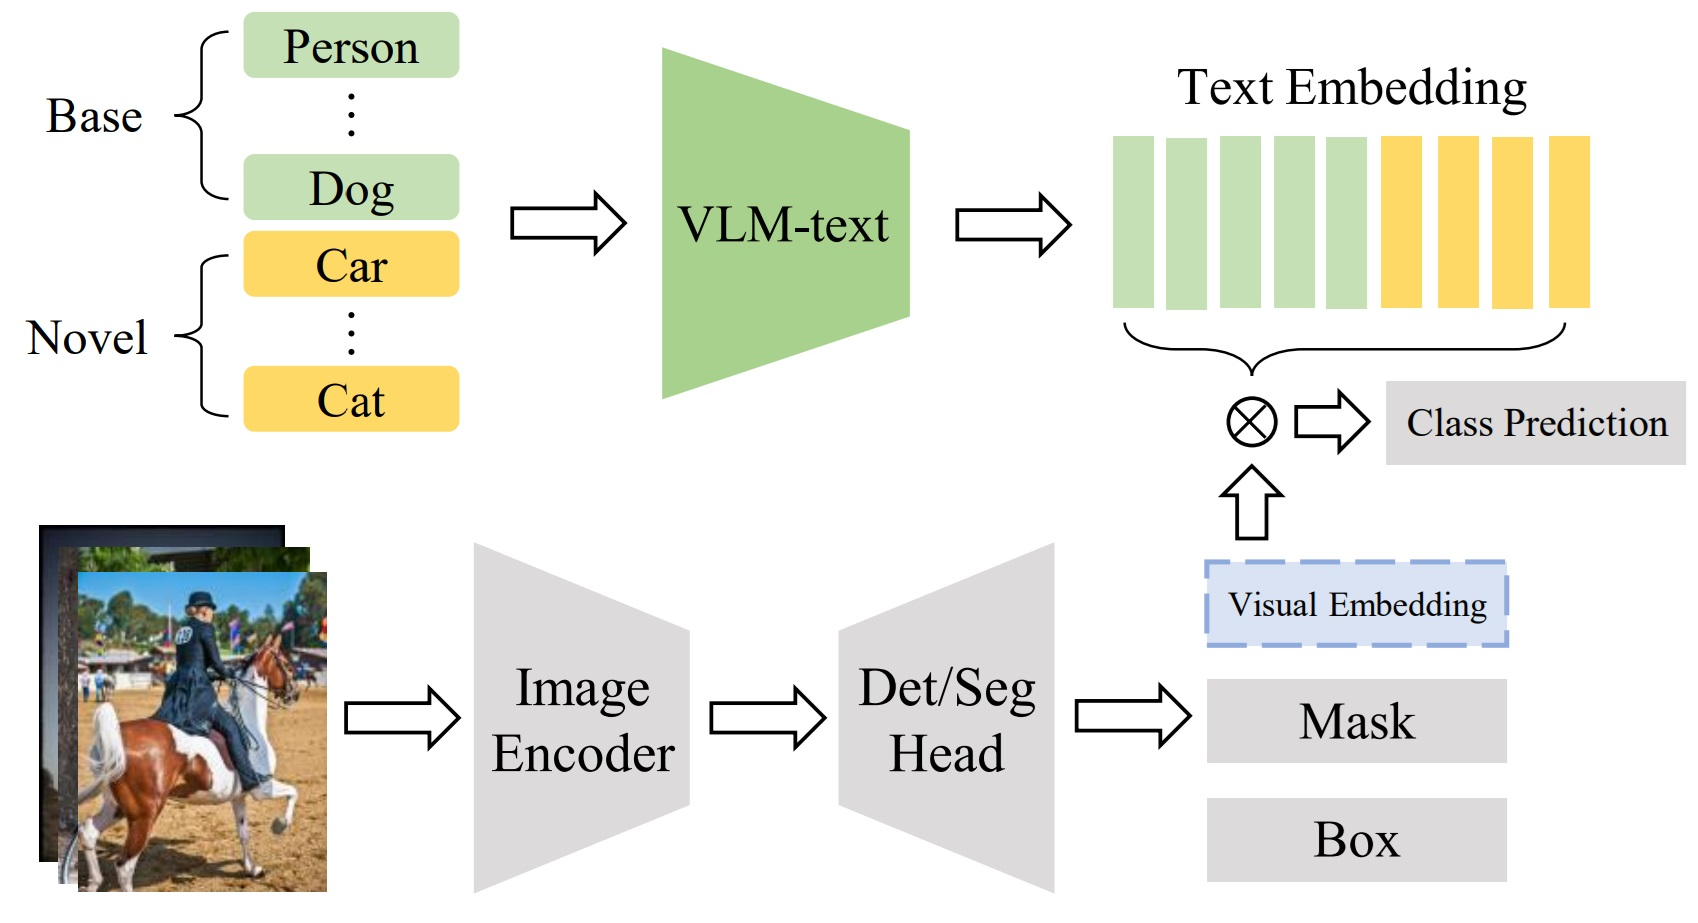
\includegraphics[width=0.55\linewidth]{PICs/tansformerSOTA/openvocabulary.jpg}
    \caption{A common structure of open vocabulary models for object detection and semantic segmentation. Vision part predicts class embeddings and VLM-text part (CLIP or ALIGN) generates class embeddings. They are compared with a dot product and the one with the highest score is the output. \cite{openvocabularysurvey2024}.}
    \label{fig:openvocabulary}
\end{figure}

The GLIP series \cite{GLIPv12022} \cite{glipv22022} are examples of such open vocabulary methods.
GLIPv2 uses a Swin Transformer \cite{swinTransformer2021} as an encoder and other transformers for text encoding.
While grounding DINO solely supports object detection tasks, GLIPv2 can be used for segmentation tasks \cite{groundingdino2024}.
The model allows object detection, instance segmentation and can perform Vision-Language understanding tasks \cite{glipv22022}.
GLIPv2 achieves comparable performance to the state-of-the-art in localization tasks.
However, inference speeds only reach up to 4.12 FPS in object detection on an NVIDIA V100.

\vspace{0.5cm}

Another intresting approach is introduced in Segment Anything \cite{segmentAnything2023} and aims to build a universal segmentation model.
Consequently, this model is trained on a dataset with over one billion masks on 11 million images.
Segment Anything \cite{segmentAnything2023} allows zero-shot detection, meaning the model can segment classes not included in training \cite{segmentAnything2023} \cite{openvocabularysurvey2024}.
\cite{segmentAnythingOnline} provides an interface to interact with this model.
Segment Anything accepts an image as an input.
The model can then segment the region of interest, which the user defines with anchor points.
\cite{segmentAnything2023} includes a prompt encoder in the model to allow such flexible prompts.
Other modules included are an image encoder, a mask decoder, and an image embedding module.
This work does not include any types of prompts in the input data.
Therefore, this model is not considered further despite achieving impressive results in segmentation tasks.
The successor model, Segment Anything 2 \cite{segmentAnything22024}, is published while finalizing this work, which solves a similar task but accepts video material as input.
The model allows object tracking in videos.
A brief experiment is conducted, applying a pre-trained SAM2 model on a rail domain video and described in the \autoref{sec:discussion} because further research is out of the scope of this work.

Table 1 in \cite{openvocabularysurvey2024} gives a detailed overview of state-of-the-art open vocabulary detection and segmentation approaches.
(hier vielleicht it includes state-of-the-art approaches like [und dann eine aufzählung]).
It lists the text models and vision models used by an approach.
Text models include CLIP \cite{CLIP2021}, BERT \cite{BERT2019}, or ALIGN \cite{ALIGN2021}, among others.
This work does not include text information in the input data, as the goal is to develop a rail track prediction system that solely bases predictions on image data.
Therefore, text models are not utilized.
The relevant parts of state-of-the-art open vocabulary approaches are the vision models.
These either consist of network architectures like Faster R-CNN or EfficientNet \cite{openvocabularysurvey2024}, which are already described in \autoref{sec:ObjectDetection} and \autoref{sec:networkArchitectures}.
Other vision models are transformer-based, like Swin Transformer \cite{swinTransformer2021}, CLIP-vision \cite{CLIP2021}, ViT \cite{ViT2021}, MaskFormer \cite{MaskFormer2021}, Mask2Former \cite{mask2Former2022}, and DINO \cite{DINO2022}.
Also commonly used MaskFormer and Mask2Former, only reach 17.6 FPS and 8.6 FPS on an NVIDIA V100 GPU \cite{mask2Former2022}.

While these open-vocabulary or universal models usually present promising approaches in terms of accuracy, most of them are transformer-based approaches and suffer from a low frame rate (below 30 FPS) \cite{carion2020endtoendobjectdetectiontransformers, groundingdino2024, swinTransformer2021, MaskFormer2021, mask2Former2022, glipv22022} making them unsuitable for real-time applications.
Therefore, they are not considered further in this work.
An additional issue is that large amounts of computing resources are often needed to train transformer-based models, which exceeds the resources of this work \cite{groundingdino2024} \cite{glipv22022}.
Also, in inference, a strong GPU is usually utilized \cite{groundingdino2024} \cite{glipv22022}.
Since the goal of this work is to be capable of real-time operation on limited embedded hardware, lightweight models are preferred.
Therefore, transformer-based models are not considered for further research.